% (c) 2012 Dimitrios Vrettos - d.vrettos@gmail.com
\chapter{I sistemi di numerazione}
\section{La scrittura in base~10}
Il nostro sistema di numerazione è il sistema \emph{decimale}. Ciò ha
probabilmente origine dal fatto che abbiamo~10 dita. Forse se fossimo
nati ragni avremmo contato fino ad otto ed useremo un sistema di
numerazione \emph{ottale}, se fossimo nati gatti avremmo contato fino a~4 e
useremo un sistema \emph{quattrale}, millepiedi fino a mille.

Come conta un
computer? Un computer ragiona sulla base di soli due stati, passa corrente (acceso) o non
passa corrente (spento): è come se avesse due dita. Tutti i sistemi che oggi
usiamo nell'informatica utilizzano una logica a due stati: i circuiti elettrici possono trovarsi nello stato di acceso o di spento, i dischi magnetici
dell'hard disk sono composti da microscopici magneti ognuno dei quali può essere magnetizzato in un verso o nel verso opposto, i dischi
ottici come i CD-ROM
e i DVD memorizzano le informazioni al loro interno come se contenessero tanti microscopici specchi ognuno dei quali riflette la luce oppure no.

Nell'antichità si usava uno strumento chiamato abaco. Gli abachi erano tavolette suddivise in colonne su cui si spalmavano
cera o sabbia e si incidevano segni o si mettevano sassolini.

Per contare un certo numero di oggetti e ricordarci quanti sono, utilizziamo un abaco:
\begin{center}
% (c) 2012 Dimitrios Vrettos - d.vrettos@gmail.com
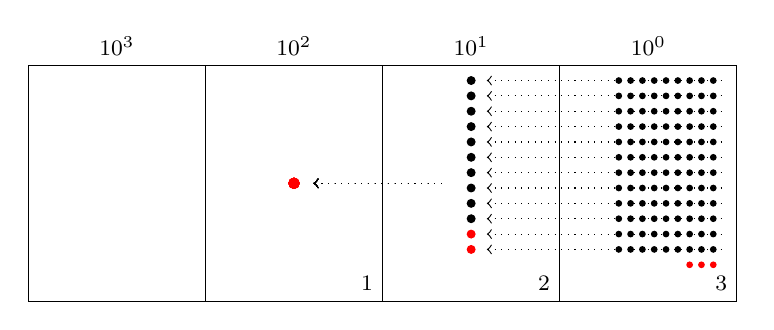
\begin{tikzpicture}[x=15mm,y=15mm, font=\footnotesize]
\foreach \x in {0,1.5,...,4.5}
\draw (\x,0) rectangle (\x+1.5,2);

\foreach \y/\ytext in {.75/$10^3$,2.25/$10^2$,3.75/$10^1$,5.25/$10^0$}
\node[above] (pot) at (\y,2) {\ytext};

\foreach \z in {1.87,1.74,...,0.44}
\foreach \a in {5,5.1,...,5.9}
\filldraw (\a,\z)circle (1pt) ;

\foreach \zi in {0.31}
\foreach \a in {5.6,5.7,5.8}
\filldraw[red] (\a,\zi)circle (1pt) ;

\foreach \zii in {1.87,1.74,...,.6}
\filldraw (3.75,\zii) circle (1.4pt);

\foreach \b in {.44,.57}
\filldraw[fill=red, draw=red] (3.75,\b) circle (1.4pt);

\foreach \yi in {1.87,1.74,...,.44}{
\node (unita) at (6,\yi) {};
\node (dec) at (3.8,\yi) {};
\draw[<-,dotted] (dec)--(unita);
\filldraw[fill=red,draw=red] (2.25,1) circle (1.8pt) node [right] (cen) {};
\draw[<-,dotted](cen)--(3.5,1);
}

\foreach \xi/\xitext in {3/1,4.5/2,6/3}
\node[left] (num) at (\xi,.15) {\xitext};

\end{tikzpicture}

\end{center}

Cominciamo a contare con le mani: per ogni raggruppamento di~10 segniamo un'unità di ordine superiore, fino a contare tutti
gli elementi del nostro insieme. Le unità che rimangono, perché non riescono a formare un raggruppamento di~10, vengono
segnate con la cifra che le rappresenta: nel nostro caso~3.

Passiamo all'unità di ordine superiore: le decine. Anche con queste formiamo raggruppamenti di~10, se ci riusciamo. Ogni
raggruppamento forma un'unità di ordine superiore, se rimangono elementi che non si raggruppano essi rappresentano le decine. Se non
rimane alcuna unità scriviamo~0. Nel nostro caso, ci sono 12~decine, 10 formano un'unità di ordine superiore (centinaia) e 2 restano decine.

Il procedimento continua finché non abbiamo finito di contare tutti gli elementi. Nel nostro esempio finiamo dopo aver formato
un'unità di ordine superiore, le centinaia. Il nostro numero è~$123$.
Ovviamente i numeri~123 e~312 sono due numeri diversi anche se composti dalle stesse cifre, sono diversi
perché la posizione delle cifre che li compongono è differente. Ad esempio, la cifra~1, che in 123 è nella posizione più a sinistra,
si trova al centro del numero~312.

Dunque, in generale, il valore attribuito alle varie cifre non dipende soltanto dalla specifica cifra considerata ma
anche dalla posizione che essa occupa all'interno del numero. Il sistema di numerazione
che solitamente usiamo è dunque un \emph{sistema posizionale}. \`E chiamato \emph{decimale} o \emph{a base
dieci} perché dieci unità di un determinato ordine sono rappresentate da un'unità di ordine superiore.

\begin{definizione}\label{def:base}
Si definisce \emph{base} di un sistema di numerazione il numero di
simboli, \emph{cifre}, usati per rappresentare i valori. La potenza della base indica il \emph{peso} (la posizione)
che i simboli hanno all'interno della scrittura del numero.
\end{definizione}

Riassumendo, abbiamo una serie di dieci simboli: 0, 1, 2, 3, 4, 5, 6, 7,
8 e 9 che rappresentano il numero delle unità di un determinato ordine.
Il significato dei simboli dipende anche dalla posizione che assumono
nella ``parola'' che rappresenta un numero.

Ad esempio:~$1\,846=1\cdot(1\,000)+8\cdot(100)+4\cdot(10)+6\cdot(1)$, che scritto con le potenze di~10 diventa:
$1\,846=1\cdot(10)^{3}+8\cdot (10)^{2}+4\cdot (10)^{1}+6\cdot (10)^{0}$.

L'esponente del peso attribuito ad ogni cifra che compone la scrittura di un numero
rappresenta la posizione della cifra a partire da quella più a destra (0) cioè la meno significativa,
quindi ne denota l'ordine di importanza.

\begin{definizione}
La scrittura di un numero come somma delle cifre moltiplicate per le potenze della
base si chiama \emph{notazione polinomiale}.
\end{definizione}

Una volta compreso il meccanismo su cui si basa il sistema
di numerazione decimale, cioè a base 10, il procedimento si può estendere ad una base
qualunque.

Se~$B$ è la base di un sistema di numerazione, $B$ unità di un certo
ordine vengono rappresentate da un'unità dell'ordine immediatamente superiore.
In questo modo si può costruire un sistema di numerazione con
qualsiasi base maggiore di~1.

\section{Scrittura di un numero in una base qualsiasi}
Il procedimento usato per scrivere un numero in base~10 può essere
usato per scrivere un numero in una base qualsiasi.

\begin{exrig}
\begin{esempio}
Contare~29 oggetti in base~5.
\begin{multicols}{2}

Utilizziamo un abaco, ma 
anziché contare per dieci contiamo per cinque. Invece di
raggruppare per unità, decine, decine di decine (centinaia) e così via,
conteremo raggruppando per unità, per cinquine, per cinquine di
cinquine (venticinquine) e così via.
\begin{center}
% (c) 2012 Dimitrios Vrettos - d.vrettos@gmail.com
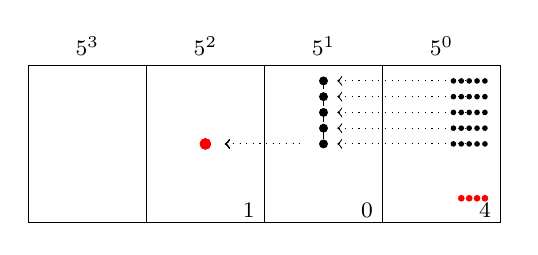
\begin{tikzpicture}[x=10mm,y=10mm, font=\footnotesize]
\foreach \x in {0,1.5,...,4.5}
\draw (\x,0) rectangle (\x+1.5,2);

\foreach \y/\ytext in {.75/$5^3$,2.25/$5^2$,3.75/$5^1$,5.25/$5^0$}
\node[above] (pot) at (\y,2) {\ytext};

\foreach \z in {1.8,1.6,...,1}
\foreach \a in {5.4,5.5,...,5.9}
\filldraw (\a,\z)circle (.8pt);
 

\foreach \zi in {0.31}
\foreach \a in {5.5,5.6,5.7,5.8}
\filldraw[red] (\a,\zi)circle (1pt) ;

\foreach \zii in {1.8,1.6,...,1}
\filldraw (3.75,\zii) circle (1.4pt);
\draw[dashed] (3.75,1.8)--(3.75,1);

\foreach \yi in {1.8,1.6,...,1}{
\node (unita) at (6,\yi) {};
\node (dec) at (3.8,\yi) {};
\draw[<-,dotted] (dec)--(unita);
\filldraw[fill=red,draw=red] (2.25,1) circle (1.8pt) node [right] (cen) {};
\draw[<-,dotted](cen)--(3.5,1);
}

\foreach \xi/\xitext in {3/1,4.5/0,6/4}
\node[left] (num) at (\xi,.15) {\xitext};

\end{tikzpicture}

\end{center}
\end{multicols}
Il numero rappresentato nell'abaco si scrive~$(104)_{5}$ e si legge
``uno-zero-quattro in base cinque'' per distinguerlo da centoquattro scritto in
base~10, che sarebbe 104 ovvero $(104)_{10}$.

Per ottenere il numero decimale che corrisponde al numero scritto in
base~5 occorre sviluppare il numero in base~5 nella sua scrittura
polinomiale:~$(104)_{5}=1\cdot 5^{2}+0\cdot 5^{1}+4\cdot5^{0}=25+0+4=(29)_{10}$.
\end{esempio}
\pagebreak
\begin{esempio}
Contare~29 oggetti in base~3.
\begin{multicols}{2}
Questa volta contiamo per tre.
Il numero ottenuto si scrive~$(1002)_{3}$ e si legge
``uno-zero-zero-due in base tre'' per distinguerlo da milledue scritto in base~10.

Per ottenere il numero decimale corrispondente, occorre sviluppare il numero in base~3 nella sua scrittura
polinomiale.
 \begin{center}
 % (c) 2012 Dimitrios Vrettos - d.vrettos@gmail.com
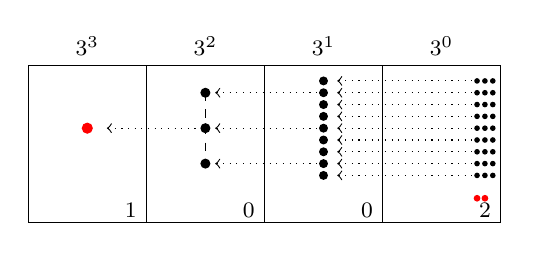
\begin{tikzpicture}[x=10mm,y=10mm, font=\footnotesize]
\foreach \x in {0,1.5,...,4.5}
\draw (\x,0) rectangle (\x+1.5,2);

\foreach \y/\ytext in {.75/$3^3$,2.25/$3^2$,3.75/$3^1$,5.25/$3^0$}
\node[above] (pot) at (\y,2) {\ytext};

\foreach \z in {1.8,1.65,...,.45}
\foreach \a in {5.7,5.8,5.9}
\filldraw (\a,\z)circle (.8pt);
 

\foreach \zi in {0.31}
\foreach \a in {5.7,5.8}
\filldraw[red] (\a,\zi)circle (1pt) ;

\foreach \zii in {1.8,1.65,...,.45}
\filldraw (3.75,\zii) circle (1.4pt);

\foreach \yi in {1.8,1.65,...,.45}{
\node (unita) at (6,\yi) {};
\node (dec) at (3.8,\yi) {};
\draw[<-,dotted] (dec)--(unita);
}
\foreach \ziii in {1.65,1.2,.75}{
\filldraw(2.25,\ziii) circle (1.6pt);
\node (cen) at (2.25,\ziii) {};
\node (deci) at (3.8,\ziii) {};
\draw[<-,dotted] (cen)--(deci);}

\draw[dashed](2.25,1.65)--(2.25,.6);

\filldraw[fill=red,draw=red] (.75,1.2) circle (1.8pt) node [right] (mig) {};
\node (ceni) at (2.25,1.2) {};
\draw[<-,dotted](mig)--(ceni);
\foreach \xi/\xitext in {1.5/1,3/0,4.5/0,6/2}
\node[left] (num) at (\xi,.15) {\xitext};

\end{tikzpicture}

 \end{center}
\end{multicols}
\[(1002)_{3}=1\cdot 3^{3}+0\cdot 3^{2}+0\cdot 3^{1}+2\cdot5^{0}=27+0+0+2=(29)_{10}.\]

\end{esempio}
\end{exrig}

In accordo con la definizione \ref{def:base}, negli esempi abbiamo visto che i simboli
che occorrono per scrivere un numero in base~10 sono
dieci~$\{$0, 1, 2, 3, 4, 5, 6, 7, 8, 9$\}$, quelli necessari per scrivere un numero
in base~5 sono cinque~$\{$0, 1, 2, 3, 4$\}$, quelli necessari per
scrivere un numero in base~3 sono tre~$\{$0, 1, 2$\}$. Analogamente, i
simboli che serviranno per scrivere un numero in base~2 sono
due~$\{$0, 1$\}$.

Possiamo scrivere i numeri anche in una base superiore a~10. Una base
molto usata in informatica, insieme alla base~2, è
la base \emph{esadecimale}, cioè la base~16.
In questo caso, per contare devo fare raggruppamenti di~16; sono
perciò necessari~16 simboli per indicare questi raggruppamenti, che rappresentano i valori da 0 a 15.
Pertanto occorrono dei simboli in più rispetto a quelli utilizzati dal sistema di numerazione decimale, che servono per rappresentare i valori~10, 11, 12, 13, 14, 15. Convenzionalmente si usano i simboli seguenti:
 \begin{align*}
 &(A)_{16}=(10)_{10}\quad (B)_{16}=(11)_{10}\quad (C)_{16}=(12)_{10}\\%
 &(D)_{16}=(13)_{10}\quad (E)_{16}=(14)_{10}\quad (F)_{16}=(15)_{10}.
 \end{align*}
Quindi i numeri esadecimali, in ordine crescente, sono: 0, 1, 2, 3, 4, 5, 6, 7, 8, 9, $A$, $B$, $C$, $D$, $E$, $F$, 10, 11, 12, 13, 14 ,15, \ldots


\subsection{Convertire un numero da una base diversa da~10 a base~10}

Per scrivere un numero da una base diversa da~10 a base~10 bisogna
svilupparlo nella sua forma polinomiale.

Se~$(x)_{B}$ è un numero qualsiasi scritto nella base~$B$ e
se~$a_{n} a_{n-1} \ldots a_{2} a_{1} a_{0}$ sono le cifre che compongono la sua rappresentazione,
da quella più significativa (con peso $B^n$) a quella meno significativa (con peso $B^0=1$), avremo:
\[(x)_{10}=a_{n}\cdot B^{n}+ a_{n-1}\cdot B^{n-1}+ \ldots%
+ a_{2}\cdot B^{2}+ a_{1}\cdot B^{1}+ a_{0}\cdot B^{0}.\]

\ovalbox{\risolvii \ref{ese:4.1}, \ref{ese:4.2}, \ref{ese:4.3}, \ref{ese:4.4}, \ref{ese:4.5}}

\subsection{Convertire un numero da base~10 a una base diversa da~10}

Abbiamo visto che per contare e scrivere un numero in una base diversa da dieci, per esempio~$(29)_{10}$ in base~3,
dobbiamo raggruppare per~3. Raggruppare per~3 ha lo stesso significato che dividere per~3. Nella
prima divisione per tre il quoziente indica quante terzine otteniamo, mentre il resto indica
quante unità (di ordine~0) verranno considerate.

\begin{multicols}{2}
Nel nostro esempio si ottengono $29/3=9$ terzine,
mentre rimangono~2 unità (di ordine~0). Il~2 sarà il primo numero a destra che verrà considerato. Con 9
terzine si ottengono $9/3=3$ terzine di terzine (novine) con resto~0. Questo~0 diventa la cifra che scriviamo
a sinistra del~2. Con 3 terzine di terzine otteniamo una terzina di terzina di terzina (ventisettina),
mentre rimangono~0 terzine di terzine. Questo~0 diventa il numero che scriviamo a sinistra dello~0 precedente. Ora,
$1:3$ dà come quoziente~0 (terzine di quarto ordine) con resto~1. Qui ci fermiamo e scriviamo~1 a sinistra dello~0
trovato precedentemente.
\begin{center}
% (c) 2012 Dimitrios Vrettos - d.vrettos@gmail.com
\begin{tikzpicture}[font=\footnotesize]

\matrix(a) [matrix of nodes,nodes={text width=19mm, text centered}]
{
Successive \emph{divisioni} per 3 &\emph{Quozienti} delle successive divisioni per 3 & \emph{Resti} delle successive divisioni per 3 \\
$29:3$&9&2\\
$9:3$&3&0\\
$3:3$&1&0\\
$1:3$&0&1\\
};
\draw[thick] (a-1-1.north west)--(a-1-3.north east);
\draw[thin] (a-2-1.north west)--(a-2-3.north east);
\draw[thick] (a-5-1.south west)--(a-5-3.south east);

\draw[->,thick,blue](a-5-3.east)--(a-2-3.east);
\end{tikzpicture}

\end{center}
\end{multicols}

Il numero si compone da sinistra verso destra con le cifre dei vari resti nell'ordine opposto a quello nel quale sono stati ottenuti. Si ha così~$(29)_{10}=(1002)_{3}$.

Controlliamo con la notazione
polinomiale:~$1\cdot 3^{3}+0\cdot3^{2}+0\cdot 3^{1}+2\cdot 3^{0}=27+2=29$.

\begin{exrig}
\begin{esempio}
Convertire nel sistema binario (in base~2) il numero~59.
\begin{multicols}{2}
Dividiamo successivamente~59 per~2 fino a che non otteniamo zero come
quoziente e prendiamo come risultato della conversione la successione
dei resti partendo dall'ultimo ottenuto.
Il numero~59 scritto in base~2 sarà pertanto~$(111011)_{2}$.

Verifichiamo con la scrittura
polinomiale:~$1\cdot 2^{5}+1\cdot2^{4}+1\cdot 2^{3}+0\cdot 2^{2}+1\cdot 2^{1}+1\cdot2^{0}=32+16+8+2+1=59$.
\begin{center}
% (c) 2012 Dimitrios Vrettos - d.vrettos@gmail.com
\begin{tikzpicture}[font=\footnotesize]

\matrix(a) [matrix of nodes,nodes={text width=19mm, text centered}]
{
Successive \emph{divisioni} per 2 &\emph{Quozienti} delle successive divisioni per 2 & \emph{Resti} delle successive divisioni per 2 \\
$59:2$&29&1\\
$29:2$&14&1\\
$14:2$&7&0\\
$7:2$&3&1\\
$3:2$&1&1\\
$1:2$&0&1\\
};
\draw[thick] (a-1-1.north west)--(a-1-3.north east);
\draw[thin] (a-2-1.north west)--(a-2-3.north east);
\draw[thick] (a-7-1.south west)--(a-7-3.south east);

\draw[->,thick,blue](a-7-3.east)--(a-2-3.east);
\end{tikzpicture}

\end{center}
\end{multicols}
\end{esempio}

\begin{esempio}
Trasforma $315$ da base~10 a base~3, 4 e 5.

% (c) 2012 Dimitrios Vrettos - d.vrettos@gmail.com
\begin{tikzpicture}[font=\small\ttfamily, matrix anchor=north]

\matrix(a) [matrix of nodes]
{
3&1&5&3\\
3&1&5&1&0&5&3\\
&&|[red]|0&1&0&5&3&5&3\\
&&&&&|[red]|0&3&3&1&1&3\\
&&&&&&&|[red]|2&&9&3&3\\
&&&&&&&&&|[red]|2&3&|[red]|1\\
&&&&&&&&&&|[red]|0&\\
};

\draw(a-1-4.north west)--(a-1-4.south west);

\draw(a-2-4.north west)--(a-2-6.north east);
\draw(a-2-7.north west)--(a-2-7.south west);
\draw(a-2-1.south west)--(a-2-3.south east);

\draw(a-3-7.north west)--(a-3-8.north east);
\draw(a-3-4.south west)--(a-3-6.south east);
\draw(a-3-9.north west)--(a-3-9.south west);

\draw(a-4-9.north west)--(a-4-10.north east);
\draw(a-4-7.south west)--(a-4-8.south east);
\draw(a-4-11.north west)--(a-4-11.south west);

\draw(a-5-11.north west)--(a-5-11.north east);
\draw(a-5-8.south east)--(a-5-10.south east);
\draw(a-5-12.north west)--(a-5-12.south west);

\draw(a-6-12.north west)--(a-6-12.north east);
\draw(a-6-11.south west)--(a-6-11.south east);

\draw[->,blue](a-7-11.south west)--(a-3-3.south west);

\node[above] (am) at (a-1-4.north) {$315_{10}=102200_3$};
\node[above] at (am.north){base 3};

\begin{scope}[xshift=45mm]
\matrix(b) [matrix of nodes]
{
3&1&5&4\\
3&1&2&7&8&4\\
&&|[red]|3&7&6&1&9&4\\
&&&&|[red]|2&1&6&4&4\\
&&&&&&|[red]|3&4&|[red]|1\\
&&&&&&&|[red]|0\\
};

 \draw(b-1-4.north west)--(b-1-4.south west);
 
 \draw(b-2-4.north west)--(b-2-5.north east);
 \draw(b-2-6.north west)--(b-2-6.south west);
 \draw(b-2-1.south west)--(b-2-3.south east);
 
\draw(b-3-6.north west)--(b-3-7.north east);
\draw(b-3-4.south west)--(b-3-5.south east);
 \draw(b-3-8.north west)--(b-3-8.south west);

\draw(b-4-8.north west)--(b-4-8.north east);
 \draw(b-4-6.south west)--(b-4-7.south east);
\draw(b-4-9.north west)--(b-4-9.south west);

 \draw(b-5-9.north west)--(b-5-9.north east);
 \draw(b-5-8.south west)--(b-5-8.south east);

 \draw[->,blue](b-6-8.south west)--(b-3-3.south west);

 \node[above] (bm) at (b-1-4.north) {$315_{10}=10323_4$};
 \node[above] at (bm.north){base 4};
\end{scope}

\begin{scope}[xshift=85mm]
\matrix(c)[matrix of nodes]
{
3&1&5&5\\
3&1&5&6&3&5\\
&&|[red]|0&6&0&1&2&5\\
&&&&|[red]|3&1&0&|[red]|2\\
&&&&&&|[red]|2\\
};

  \draw(c-1-4.north west)--(c-1-4.south west);
  
\draw(c-2-4.north west)--(c-2-5.north east);
\draw(c-2-6.north west)--(c-2-6.south west);
\draw(c-2-1.south west)--(c-2-3.south east);

\draw(c-3-6.north west)--(c-3-7.north east);
\draw(c-3-4.south west)--(c-3-5.south east);
 \draw(c-3-8.north west)--(c-3-8.south west);
 
 \draw(c-4-8.north west)--(c-4-8.north east);
 \draw(c-4-6.south west)--(c-4-7.south east);

 \draw[->,blue](c-5-7.south west)--(c-3-3.south west);

 \node[above] (cm) at (c-1-4.north) {$315_{10}=2230_5$};
 \node[above] at (cm.north){base 5};
\end{scope}
\end{tikzpicture}

\end{esempio}
\end{exrig}

\subsubsection{Un altro metodo per trasformare un numero decimale in un numero binario}

Per trasformare i numeri da base~10 a base~2 basta scrivere il numero
come somma delle potenze del~2:
\begin{enumeratea}
\item si parte dalla potenza del~2 più vicina, per difetto, al numero da convertire;
\item si vede se la potenza precedente di ordine inferiore può fare parte della sequenza, cioè se la somma tra
le potenze non diventa più grande del numero. Se può farne parte allora si scrive~1, altrimenti~0;
\item si prosegue in questo modo fino ad arrivare a~$2^{0}$;
\item la sequenza di~1 e~0 nell'ordine ottenute sono le cifre che, da sinistra verso destra, rappresentano il numero binario corrispondente.
\end{enumeratea}

\begin{exrig}
\begin{esempio}
Consideriamo ancora il numero~59:
\begin{itemize*}
\item qual è la potenza del~2 più vicina, per difetto, al numero~59? \`E~32, cioè~$2^{5}$. Quindi~$2^{5}$
fa parte del numero binario. Scrivo~1 come primo numero della sequenza;
\item vediamo ora~$2^{4}=16$. Anche~16 può far parte del numero binario perché~$32 + 16 = 48$ che è minore di~59.
Segno~1 come secondo numero della sequenza;
\item per lo stesso ragionamento anche~$2^{3}=8$ fa parte del numero binario.
Infatti~$32 + 16 + 8 = 56$ è minore di~59. Segno ancora~1 come terzo numero della sequenza;
\item invece~$2^{2}=4$ non può farne parte perché $32 + 16 + 8 + 4 = 60$ è maggiore di~59. Segno~0 come quarto numero
della sequenza;
\item $2^{1}=2$ e~$2^{0}=1$ vanno bene e si arriva al totale voluto~59. Segno~1 come quinto e~1 come sesto numero
della sequenza.
\end{itemize*}
Riassumendo:~$59=1\cdot 2^{5}+1\cdot 2^{4}+1\cdot2^{3}+0\cdot 2^{2}+1\cdot 2^{1}+1\cdot2^{0}=(111011)_{2}$.
\end{esempio}
\end{exrig}

\ovalbox{\risolvii{\ref{ese:4.6}, \ref{ese:4.7}, \ref{ese:4.8}, \ref{ese:4.9}, \ref{ese:4.10}, \ref{ese:4.11}, \ref{ese:4.12},
\ref{ese:4.13}, \ref{ese:4.14}}}

\section[Conversione da una base diversa da~10 a un'altra base diversa da~10]{Conversione di un numero da una base diversa da~10 a un'altra base diversa da~10}
\begin{exrig}
\begin{esempio}
Scrivere il numero~$(1023)_{4}$ in base~7.

Per scrivere un numero da una base~$B$ a una base~$K$ entrambe diverse da~10 occorre:

\begin{enumeratea}
\item trasformare il numero in base~$B$ in un numero decimale attraverso
la sua scrittura polinomiale;

$(1023)_{4}\;=\;1\cdot 4^{3}\;+\;0\cdot 4^{2}\;+\;2\cdot 4^{1}\;+\;3\cdot
4^{0}\;=\;64\;+\;0\;+\;8\;+\;3\;=\;(75)_{10}$;
\item trasformare il numero decimale nella base~$K$ attraverso i resti
delle divisioni successive per~$K$ presi nell'ordine opposto a quello nel quale sono stati ottenuti.
\begin{center}
 % (c) 2012 Dimitrios Vrettos - d.vrettos@gmail.com
\begin{tikzpicture}[font=\small]

\matrix(a) [matrix of nodes,nodes={text width=25mm, text centered}]
{
Successive \emph{divisioni} per 7 &\emph{Quozienti} delle successive divisioni per 7 & \emph{Resti} delle successive divisioni per 7 \\
$75:7$&10&5\\
$10:7$&1&3\\
$1:7$&0&1\\
};
\draw[thick] (a-1-1.north west)--(a-1-3.north east);
\draw[thin] (a-2-1.north west)--(a-2-3.north east);
\draw[thick] (a-4-1.south west)--(a-4-3.south east);

\draw[->,thick,blue](a-4-3.east)--(a-2-3.east);
\end{tikzpicture}

\end{center}
\end{enumeratea}
\begin{comment}
Applichiamo la procedura indicata:

\begin{enumeratea}
\item
$(1023)_{4}\;=\;1\cdot 4^{3}\;+\;0\cdot 4^{2}\;+\;2\cdot 4^{1}\;+\;3\cdot
4^{0}\;=\;64\;+\;0\;+\;8\;+\;3\;=\;(75)_{10}$;
\item Il numero scritto da sinistra verso destra con i resti delle successive
divisioni per~7 presi nell'ordine opposto a quello nel quale sono stati ottenuti è
$(135)_{7}$.
\end{enumeratea}

\begin{center}
 % (c) 2012 Dimitrios Vrettos - d.vrettos@gmail.com
\begin{tikzpicture}[font=\small]

\matrix(a) [matrix of nodes,nodes={text width=25mm, text centered}]
{
Successive \emph{divisioni} per 7 &\emph{Quozienti} delle successive divisioni per 7 & \emph{Resti} delle successive divisioni per 7 \\
$75:7$&10&5\\
$10:7$&1&3\\
$1:7$&0&1\\
};
\draw[thick] (a-1-1.north west)--(a-1-3.north east);
\draw[thin] (a-2-1.north west)--(a-2-3.north east);
\draw[thick] (a-4-1.south west)--(a-4-3.south east);

\draw[->,thick,blue](a-4-3.east)--(a-2-3.east);
\end{tikzpicture}

\end{center}
\end{comment}

Le trasformazioni eseguite
sono quindi:~$(1023)_{4}\rightarrow (75)_{10}\rightarrow (135)_{7}$.

\end{esempio}
\end{exrig}

\ovalbox{\risolvii \ref{ese:4.15}, \ref{ese:4.16}, \ref{ese:4.17}}

\subsection{Conversione tra base~4, base~8, base~16 e base~2}

Consideriamo il numero scritto in base~2 $(11010011100101)_{2}$.
Vogliamo scriverlo in base~4, in base~8, in base~16 senza passare dalla
sua scrittura in base~10. Notiamo che gruppi di due cifre in base~2
rappresentano tutte le cifre della base~4, gruppi di~3 cifre in base~2
rappresentano tutte le cifre della base~8 e gruppi di~4 cifre nella
base~2 rappresentano tutte le cifre della base~16, come indicato nella
seguente tabella.

\begin{center}
 \begin{tabular*}{.7\textwidth}{@{\extracolsep{\fill}}*{5}{c}}
\toprule
Base~10 & Base~2 & Base~4 & Base~8 & Base~16\\
\midrule
 0 & 0 & $00 = 0$ & $000 = 0$ & $0000 = 0$\\
 1 & 1 & $01 = 1$ & $001 = 1$ & $0001 = 1$\\
 2 &   & $10 = 2$ & $010 = 2$ & $0010 = 2$\\
 3 &   & $11 = 3$ & $011 = 3$ & $0011 = 3$\\
 4 &   &          & $100 = 4$ & $0100 = 4$\\
 5 &   &          & $101 = 5$ & $0101 = 5$\\
 6 &   &          & $110 = 6$ & $0110 = 6$\\
 7 &   &          & $111 = 7$ & $0111 = 7$\\
 8 &   &          &           & $1000 = 8$\\
 9 &   &          &           & $1001 = 9$\\
10 &   &          &           & $1010 = A$\\
11 &   &          &           & $1011 = B$\\
12 &   &          &           & $1100 = C$\\
13 &   &          &           & $1101 = D$\\
14 &   &          &           & $1110 = E$\\
15 &   &          &           & $1111 = F$\\
\bottomrule
 \end{tabular*}
\end{center}

\paragraph{Da base~2 a base~4}
Dobbiamo raggruppare il numero scritto in base~2 in gruppi di due cifre, partendo da destra, e tradurre il valore di ogni singolo gruppo con la
corrispondente cifra in base~4.

\begin{tabular*}{.9\textwidth}{@{\extracolsep{\fill}}*{8}{c}}
\toprule
Numero scritto in base~2 & 1 1 & 0 1 & 0 0 & 1 1 & 1 0 & 0 1 & 0 1\\
Numero scritto in base~4 &  3  &  1  &  0  &  3  &  2  &  1  &  1\\
\bottomrule
\end{tabular*}
\[(11010011100101)_{2}=(3103211)_{4}.\]

\paragraph{Da base~2 a base~8}
Dobbiamo raggruppare il numero scritto in base~2 in gruppi di tre cifre, partendo da destra,
e tradurre il valore di ogni singolo gruppo con la corrispondente cifra in base~8.

\begin{tabular*}{.9\textwidth}{@{\extracolsep{\fill}}*{6}{c}}
\toprule
 Numero scritto in base~2 & 1 1 & 0 1 0 & 0 1 1 & 1 0 0 & 1 0 1\\
 Numero scritto in base~8 &  3  &   2   &   3   &   4   &   5\\
 \bottomrule
\end{tabular*}
\[(11010011100101)_{2}=(32345)_{8}.\]

\paragraph{Da base~2 a base~16}
Dobbiamo raggruppare il numero scritto in base~2 in gruppi di quattro cifre, partendo da destra,
e tradurre il valore di ogni singolo gruppo con la corrispondente cifra in base~16.

\begin{tabular*}{.9\textwidth}{@{\extracolsep{\fill}}*{5}{c}}
\toprule
 Numero scritto in base~2  & 1 1 & 0 1 0 0 & 1 1 1 0 & 0 1 0 1\\
 Numero scritto in base~16 &  3  &    4    &   $E$   &    5\\
 \bottomrule
\end{tabular*}
\[(11010011100101)_{2}=(34E5)_{16}.\]

\ovalbox{\risolvii \ref{ese:4.18}, \ref{ese:4.19}}

\subsubsection{Perché è importante la base~2?}

Tutti gli strumenti elettronici che utilizziamo hanno bisogno di
tradurre le informazioni che inseriamo in stati fisici della
macchina. Dal punto di vista tecnico oggi usiamo dispositivi elettrici, magnetici, ottici che sono bistabili, ossia assumono due stati fisici differenti e il metodo più semplice e più efficiente per tradurre in ``linguaggio macchina''
le nostre informazioni è utilizzare la base~2: composta solo dai
simboli~0 e~1. La base due è quindi l'alfabeto a
disposizione delle macchine per comprendere e rispondere alle nostre
richieste. Se si utilizzasse la base~10 dovremo far riconoscere
dall'apparato dieci differenti simboli che dovrebbero
essere tradotti in altrettanti stati differenti di dispositivi fisici.

A partire da questa informazione elementare detta \textit{bit}
(compressione dall'inglese di \textit{bi}nary
digi\textit{t}) è possibile costruire informazioni più complesse
sotto forma di sequenze finite di zero e di uno. Attraverso la codifica
binaria si è in grado di rappresentare caratteri, numeri, istruzioni
di programmi ma anche immagini, suoni e video. Tutte le informazioni
gestite da un computer sono quindi numeri in forma binaria.

Il primo multiplo del bit è il \textit{byte} che è formato da una
sequenza di~8 bit:
 \begin{center}
% (c) 2012 Dimitrios Vrettos - d.vrettos@gmail.com
\begin{tikzpicture}[font=\ttfamily]

\matrix(a) [matrix of nodes,nodes={draw, text centered}]
{
0&1&0&1&0&0&0&0 \\
};

\end{tikzpicture}

 \end{center}

Con una sequenza di~8 bit possiamo codificare, per mezzo del codice ASCII\footnote{Acronimo di \textit{American Standard Code for Information Interchange}. Si tratta di un codice standard utilizzato dalla maggior parte dei sistemi elettronici per associare ogni lettera alfanumerica a un valore numerico.}, fino a~256 caratteri. Quando digitiamo un carattere sulla
tastiera del calcolatore inviamo in realtà una sequenza di~8 bit.
Vediamo alcuni esempi della codifica binaria dei caratteri (codice ASCII).

\begin{table}[!h]
\begin{center}
\begin{tabular}{ccc}
\toprule
Carattere & In base~2 & Numero decimale\\
\midrule
A & 0 1 0 0 0 0 0 1 & 65\\
a & 0 1 1 0 0 0 0 1 & 97\\
M & 0 1 0 0 1 1 0 1 & 77\\
m & 0 1 1 0 1 1 0 1 & 109\\
0 & 0 0 1 1 0 0 0 0 & 48\\
1 & 0 0 1 1 0 0 0 1 & 49\\
à & 1 0 1 0 0 0 0 0 & 160\\
ò & 1 0 1 0 0 0 1 0 & 162\\
\bottomrule
\end{tabular}
\end{center}
\end{table}
\pagebreak
Anche il byte ha i suoi multipli. Eccone alcuni indicati nelle seguenti tabelle.

\begin{table}[!h]
\begin{center}
{\small
\begin{tabular}{llcr}
\toprule
\multicolumn{4}{c}{Sistema internazionale}\\
Nome & Simbolo & Potenza di~10 & Valore decimale rispetto al byte\\
\midrule
byte      & $\unit{B}$  & $10^{0}$  & 1\\
kilobyte  & $\unit{kB}$ & $10^{3}$  & \np{1000}\\
megabyte  & $\unit{MB}$ & $10^{6}$  & \np{1000000}\\
gigabyte  & $\unit{GB}$ & $10^{9}$  & \np{1000000000}\\
terabyte  & $\unit{TB}$ & $10^{12}$ & \np{1000000000000}\\
petabyte  & $\unit{PB}$ & $10^{15}$ & \np{1000000000000000}\\
exabyte   & $\unit{EB}$ & $10^{18}$ & \np{1000000000000000000}\\
zettabyte & $\unit{ZB}$ & $10^{21}$ & \np{1000000000000000000000}\\
yottabyte & $\unit{YB}$ & $10^{24}$ & \np{1000000000000000000000000}\\
\bottomrule
\end{tabular}}
\end{center}
\end{table}

\begin{table}[!h]
\begin{center}
{\small
\begin{tabular}{llcr}
\toprule
\multicolumn{4}{c}{Utilizzo in informatica}\\
Nome & Simbolo & Potenza di~2 & Valore decimale rispetto al byte\\
\midrule
byte     & $\unit{B}$   & $2^{0}$  & 1\\
kibibyte & $\unit{KiB}$ & $2^{10}$ & \np{1024}\\
mebibyte & $\unit{MiB}$ & $2^{20}$ & \np{1048576}\\
gibibyte & $\unit{GiB}$ & $2^{30}$ & \np{1073741824}\\
tebibyte & $\unit{TiB}$ & $2^{40}$ & \np{1099511627776}\\
pebibyte & $\unit{PiB}$ & $2^{50}$ & \np{1125899906842624}\\
exbibyte & $\unit{EiB}$ & $2^{60}$ & \np{1152921504606846976}\\
zebibyte & $\unit{ZiB}$ & $2^{70}$ & \np{1180591620717411303424}\\
yobibyte & $\unit{YiB}$ & $2^{80}$ & \np{1208925819614629174706176}\\
\bottomrule
\end{tabular}}
\end{center}
\end{table}


\osservazione È noto che i prefissi \textit{kilo-}, \textit{mega-} e \textit{giga-}
corrispondono a~$\np{1000}$, $\np{1000000}$ (un milione) e~$\np{1000000000}$ (un
miliardo), mentre nell'informatica vengono
impropriamente usati per indicare particolari potenze di~2 (\textit{kibi-}, \textit{mebi-} e \textit{gibi-}).
Tutto questo genera confusione e i produttori giocano su questa
differenza, facendo i conti con i multipli decimali, ``imbrogliando''. Un PC che
viene dichiarato, ad esempio, con un hard disk da~$160\unit{GB}$ ha a disposizione~$160\cdot 10^{9}$ byte che risultano essere $160\cdot(10^9 / 2^{30}) = 160 \cdot \np{0,931322575} \simeq 149\unit{GiB}$\@. Ma il PC gestisce i multipli binari, ovvero i $\unit{GiB}$, e quindi mostra all'utente un disco da $149\unit{GiB}$\@. Ecco che ci siamo ``persi'' circa~$160-149=11\unit{GiB}$.

\vspazio\ovalbox{\risolvi \ref{ese:4.20}}

\section{Operazioni in base diversa da dieci}

Le quattro operazioni con i numeri in base diversa da dieci possono
effettuarsi con gli stessi algoritmi utilizzati per i numeri naturali.
\pagebreak
\subsection{Addizione}

\begin{exrig}
\begin{esempio}
Eseguire l'addizione in base~2 tra~$101011_{2}$ e~$10011_{2}$.
\end{esempio}

Dobbiamo tradurre in base due quello che facciamo in base dieci. Abbiamo
perciò bisogno di costruire la tavola di addizione in base due che
riportiamo a lato. La tavola, o tabellina, è piuttosto semplice,
bisogna solo fare attenzione che in base due si ha~$1+1=10$, perché in base due il~2 si scrive appunto~10.

\begin{wrapfloat}{figure}{r}{0pt}
% (c) 2012 Dimitrios Vrettos - d.vrettos@gmail.com
\begin{tikzpicture}[font=\small\ttfamily,anchor=north]

\matrix(a) [matrix of nodes,nodes={ text centered}]
{
+&0&1\\
0&0&1 \\
1&1&10\\
};
\begin{scope}[blue]
\draw (a-1-2.north west)--(a-3-2.south west);
\draw (a-2-1.north west) -- (a-2-3.north east);
\end{scope}
\begin{scope}[xshift=35mm]
\matrix(b) [matrix of nodes,nodes={ text centered },cells={anchor=north}, row 1/.style={red}]
{
Riporti&&&&1&1\\
&1&0&1&0&1&1&$+$ \\
&&1&0&0&1&1&{}\\
&1&1&1&1&1&0\\
};
\draw (b-4-2.north west)--(b-4-7.north east);
\end{scope}
\end{tikzpicture}

\end{wrapfloat}

Mettiamo i numeri in colonna e cominciamo ad addizionare
a partire dalle unità:~$1+1=0$, scrivo~$0$ e riporto~$1$.
Nella colonna di ordine superiore troviamo~$(1+1)+1=10+1=11$, scrivo~$1$ e
riporto~$1$.
Nella colonna di ordine superiore troviamo~$1+0+0=1$, scrivo~$1$ senza
riportare alcunché. Continuo in questo modo fino ad esaurire tutte le cifre da addizionare.

Facciamo la verifica nel sistema decimale:
%\[(101011_{2}=43)+(10011_{2}=19)=(111110_{2}=62).\]
\begin{align*}
&\text{in base 2 }&101011_{2}&+10011_{2}&=&~111110_{2}\\
&\text{in base 10 }&43&+19&=&~62
\end{align*}
\begin{esempio}
Eseguire la somma in base~5 tra~$34231_{5}$ e~$4341_{5}$.

Costruiamo la tavola di addizione in base cinque: ricordiamo che~$4+1=10$, $4+2=11$, $4+3=12$ ecc.

Mettiamo i numeri in colonna e cominciamo ad addizionare a partire dalle
unità:~$1+1=2$, scrivo~$2$ senza riporto. Nella colonna di ordine superiore
troviamo~$3+4=12$. Scrivo~$2$ e riporto~$1$. Nella colonna di ordine superiore troviamo~$(1+2)+3=3+3=11$ scrivo~$1$ e
riporto~$1$. Procedendo verso sinistra ora troviamo~$(1+4)+4=10+4=14$ scrivo~$4$ e
riporto~$1$. Infine~$1+3=4$. L'addizione è terminata.
%\newpage
\begin{center}
 % (c) 2012 Dimitrios Vrettos - d.vrettos@gmail.com
\begin{tikzpicture}[font=\small\ttfamily, anchor=north, x=6mm, y=6mm]

  \node (o) at (0,0) {$+$}; 
  \foreach \x in {0,1,...,4} { 
    \node (a) at (\x+1,0) {\x}; 
    \node (b) at (0,-\x-1) {\x}; 
  }

  \foreach \x[count=\xi] in {0,...,4} 
    \foreach \y [count={\yi+6}]in {\x,...,4}
      \node () at (\xi,-\yi) {\y};

   \foreach \x[count=\xii] in {10,...,13} 
     \foreach \y [count=\yii]in {\x,...,10}
       \node () at (\xii+1,\yii-6) {\y};

\begin{scope}[blue]
  \draw (-3mm,-6mm)--(33mm,-6mm); 
  \draw (3mm,0mm)--(3mm,-35mm); 
\end{scope}

\begin{scope}[xshift=65mm]
\matrix(b) [matrix of nodes,nodes={ text centered },cells={anchor=north}, row 1/.style={red}]
{
Riporti&1&1&1&&\\
&3&4&2&3&1&$+$ \\
&&4&3&4&1&\\
&4&4&1&2&2\\
};
\draw (b-4-2.north west)--(b-4-6.north east);
\end{scope}

\end{tikzpicture}

\end{center}
Verifica nel sistema decimale:
%\[(34231_{5}=2\,441)\;+\;(4341_{5}=596)=(44122_{5}=3\,037).\]
\begin{align*}
&\text{in base 5 }&34231_{5}&+4341_{5}&=&~44122_{5}\\
&\text{in base 10 }&2\,441&+596&=&~3\,037
\end{align*}
\end{esempio}

\end{exrig}

\ovalbox{\risolvii \ref{ese:4.21}, \ref{ese:4.22}, \ref{ese:4.23}}
\pagebreak
\subsection{Sottrazione}

Per la sottrazione ci possiamo servire delle stesse tabelle
dell'addizione.

\begin{exrig}
\begin{esempio}
$101011_{2}-11111_{2}.$
\end{esempio}

Mettiamo i numeri in colonna e cominciamo a sottrarre partendo dalle
unità:~$1-1=0$ scrivo~$0$.
Nella colonna di ordine superiore troviamo di nuovo~$1-1=0$ scrivo~$0$.
Procedendo verso sinistra troviamo~$0-1$ devo quindi prendere in prestito
un unità di ordine superiore che messa davanti a~0 diviene~$10-1=1$.
Scrivo~$1$ e riporto~$-1$. Mi sposto ancora a sinistra e
\begin{wrapfloat}{figure}{r}{0pt}
 % (c) 2012 Dimitrios Vrettos - d.vrettos@gmail.com
\begin{tikzpicture}[font=\small\ttfamily]


\matrix(b) [matrix of nodes,nodes={ text centered },cells={anchor=north}, row 1/.style={red}]
{
Riporti&-1&-1&-1&&\\
&1&0&1&0&1&1&$-$ \\
&&1&1&1&1&1&{}\\
&0&0&1&1&0&0\\
};
\draw (b-4-2.north west)--(b-4-7.north east);

\end{tikzpicture}

\end{wrapfloat}
trovo~$(-1+1)-1=0-1$. Occorre prendere in
prestito un'unità di ordine superiore~$10-1=1$.
Scrivo~$1$ e riporto~$-1$.
Nella colonna a sinistra ho~$0$ del minuendo, $-1$ del riporto e~$-1$
del sottraendo. Occorre prendere a prestito un'unità
di ordine superiore quindi~$10-1=1$ a cui devo togliere~$1$ del
sottraendo:~$1-1=0$.
Infine nella unità di ordine superiore devo addizionare il riporto
$-1$ a~$1$ e scrivo ancora~$0$. Il risultato della sottrazione è:~$1100_2$

Verifica nel sistema decimale: %~$(101011_{2}=43)-(11111_{2}=31)=(1100_{2}=12).$
\begin{align*}
&\text{in base 2 }&101011_{2}&-11111_{2}&=&~1100_{2}\\
&\text{in base 10 }&43&-31&=&~12
\end{align*}


\begin{esempio}
$34231_{5}-4341_{5}.$

Ci serviamo della tavola di addizione in base cinque.
\begin{center}
 \input{./lbr/chap04/fig015_sot.pgf}
\end{center}
Verifica nel sistema decimale: %~$(34231_{5}=2\,441)-(4341_{5}=596)=(24340_{5}=1\,845).$
\begin{align*}
&\text{in base 5 }&34231_{5}&-4341_{5}&=&~24340_{5}\\
&\text{in base 10 }&2\,441&+596&=&~1\,845
\end{align*}
\end{esempio}
\end{exrig}

\ovalbox{\risolvii \ref{ese:4.24}, \ref{ese:4.25}, \ref{ese:4.26}}
\pagebreak
\subsection{Moltiplicazione}

Adoperiamo lo stesso algoritmo usato per moltiplicare due numeri
decimali utilizzando la tabella della moltiplicazione.

\begin{exrig}

\begin{esempio}
$101011_{2}\cdot~101_{2}.$

Dobbiamo tradurre in base due quello che facciamo in base dieci. Abbiamo
perciò bisogno di costruire la tavola della moltiplicazione in base
due.
\begin{center}
% (c) 2012 Dimitrios Vrettos - d.vrettos@gmail.com
\begin{tikzpicture}[font=\small\ttfamily,anchor=north]

\matrix(a) [matrix of nodes,nodes={ text centered}]
{
$\cdot$&0&1\\
0&0&0 \\
1&0&1\\
};
\begin{scope}[blue]
\draw (a-1-2.north west)--(a-3-2.south west);
\draw (a-2-1.north west) -- (a-2-3.north east);
\end{scope}
\begin{scope}[xshift=35mm]
\matrix(b) [matrix of nodes,nodes={ text centered },cells={anchor=north}]
{

&&1&0&1&0&1&1&$\cdot$ \\
{}&&&&&1&0&1&{}\\
&&1&0&1&0&1&1\\
&0 & 0 & 0 & 0 & 0 & 0&$-$\\
 1 & 0 & 1 & 0 & 1 & 1&$-$ \\
1&1&0&1&0&1&1&1\\
};
\draw (b-3-3.north west)--(b-3-8.north east);
\draw (b-6-1.north west)--(b-6-8.north east);
\end{scope}
\end{tikzpicture}

\end{center}
Verifica nel sistema decimale: %~$(101011_{2}=43)\cdot(101_{2}=5)=(11010111_{2}=215)$.
\begin{align*}
&\text{in base 2 }&101011_{2}&\cdot 101_{2}&=&~11010111_{2}\\
&\text{in base 10 }&43&\cdot 5&=&~215
\end{align*}
 \end{esempio}
%\pagebreak
 \begin{esempio}
 $231_{5}\times~24_{5}$.

In questo caso abbiamo bisogno di costruire la tavola della moltiplicazione in base
cinque.

\begin{center}
 % (c) 2012 Dimitrios Vrettos - d.vrettos@gmail.com
\begin{tikzpicture}[font=\small\ttfamily,anchor=north]

\matrix(a) [matrix of nodes,nodes={ text centered}]
{
$\cdot$&0&1&2&3&4\\
0&0&0&0&0&0 \\
1&0&1&2&3&4\\
2&0&2&4&11&13\\
3&0&3&11&14&22\\
4&0&4&13&22&31\\
};
\begin{scope}[blue]
\draw (a-1-2.north west)--(a-6-2.south west);
\draw (a-2-1.north west) -- (a-2-6.north east);
\end{scope}
\begin{scope}[xshift=45mm]
\matrix(b) [matrix of nodes,nodes={ text centered },cells={anchor=north}]
{

&&2&3&1&$\cdot$ \\
{}&&&2&4\\
{}&2&0&2&4\\
1&0&1&2&-&\\
 1 & 2 & 1 & 4 &4 \\
};
 \draw (b-3-2.north west)--(b-3-5.north east);
\draw (b-5-1.north west)--(b-5-5.north east);
\end{scope}
\end{tikzpicture}

\end{center}
 Verifica nel sistema decimale: %~$(231_{5}=66)\cdot(24_{5}=14)=(12144_{5}=924)$.
\begin{align*}
&\text{in base 5 }&231_{5}&\cdot 24_{5}&=&~12144_{5}\\
&\text{in base 10 }&66&\cdot 14&=&~924
\end{align*}
 \end{esempio}
\end{exrig}

\ovalbox{\risolvii \ref{ese:4.27}, \ref{ese:4.28}, \ref{ese:4.29}}
\pagebreak
\subsection{Divisione}

Anche per la divisione il procedimento è del tutto analogo a quello
usato nel sistema decimale, la tavola da utilizzare è quella della
moltiplicazione.

\begin{exrig}

\begin{esempio}
$11101_{2}:101_{2}.$
\end{esempio}
Dobbiamo tradurre in base due quello che facciamo in base dieci.

\begin{wrapfloat}{figure}{r}{0pt}
% (c) 2012 Dimitrios Vrettos - d.vrettos@gmail.com
\begin{tikzpicture}[font=\small\ttfamily,anchor=north]

\matrix(a) [matrix of nodes,nodes={ text centered}]
{
&1  & 1  & 1  & 0  & 1 & 1 & 0 & 1\\
$-$&1 & 0 & 1 & & & 1 & 0 & 1\\
&& 1  & 0  & 0  &\\
& & 0 & 0 & 0 \\
& & 1 & 0 & 0 & 1\\
& &  $-$&1 & 0 & 1 &\\
& & & 1 & 0 & 0 &\\
};

 \draw (a-1-7.north west)--(a-2-7.south west);
\draw (a-2-7.north west) -- (a-2-9.north east);
\draw (a-2-2.south west) -- (a-2-4.south east);
\draw (a-4-3.south west) -- (a-4-5.south east);
\draw (a-6-4.south west) -- (a-6-6.south east);
\end{tikzpicture}

\end{wrapfloat}

La cifra di ordine più alto si ottiene dalla divisione di~$111$ con~$101$.
Il quoziente è~$1$, il resto si ottiene dalla differenza tra
il dividendo e il prodotto del quoziente per il divisore. In questo
caso il resto è~$10$.

Si abbassa lo~$0$ e otteniamo~$100$. Si ha~$100:101=0$. La seconda
cifra del divisore è~$0$.

La moltiplicazione di~$0$ per il divisore dà~$0$. Il nuovo resto è~$100$.

Si abbassa l'1 e otteniamo~$1001$ che viene diviso per~$101$. Il quoziente è~$1$
ed il resto è uguale a~$100$.

Dai calcoli risulta quindi: $11101_{2}:101_{2} = (101)_2$ con resto $(100)_2$.

Verifica nel sistema decimale:
%\[(11101_{2}=29):(101_{2}=5)=(\mathit{Quoziente}:101_{2}=5;\:\:\mathit{Resto}:110_{2}=4).\]
\begin{align*}
&\text{in base 2 }&11101_{2}&:101_{2}&=&~101_{2}&\text{con Resto }=&~100_{2}\\
&\text{in base 10 }&29&:5&=&~5&\text{con Resto }= &~4
\end{align*}

%\begin{multicols}{2}
\begin{wrapfloat}{figure}{r}{0pt}
% (c) 2012 Dimitrios Vrettos - d.vrettos@gmail.com
\begin{tikzpicture}[font=\small\ttfamily,anchor=south]

\matrix(a) [matrix of nodes,nodes={ text centered}]
{
&&1  & 0  & 1 & $\cdot$\\
&&1 & 0 & 1 \\
&&1  & 0  & 1 &\\
 & 0 & 0 & 0&$-$ \\
 1 & 0  & 1&$-$\\
1 & 1& 0 &0&1\\
};

\draw (a-3-3.north west) -- (a-3-5.north east);
\draw (a-6-1.north west) -- (a-6-5.north east);

\begin{scope}[xshift=25mm]
\matrix(b) [matrix of nodes,nodes={ text centered}]
{
1  &1&0& 0  & 1 & $+$\\
&&1 & 0 & 0 \\
1&1&1  & 0  & 1 &\\
};
\end{scope}
\draw (b-3-1.north west) -- (b-3-5.north east);
\end{tikzpicture}

\end{wrapfloat}
Eseguiamo la riprova della divisione in base~2:
\[\mathit{dividendo}=\mathit{quoziente}\cdot\mathit{divisore}+\mathit{resto}.\]
Il quoziente $101_2$ moltiplicato per il divisore $101_2$ è uguale a~$11001_2$.
Se a questo risultato aggiungiamo il resto~$100_2$ otteniamo il dividendo~$11101_2$. Quindi i calcoli effettuati sono corretti.

%\end{multicols}
%\pagebreak
\begin{esempio}
$3402_{5}:42_{5}$.
\end{esempio}

\begin{wrapfloat}{figure}{r}{0pt}
 % (c) 2012 Dimitrios Vrettos - d.vrettos@gmail.com
\begin{tikzpicture}[font=\small\ttfamily,anchor=south]

\matrix(a) [matrix of nodes,nodes={ text centered}]
{
3&4  & 0  & 2 & 4&2\\
3 & 2 & 3 &{}&4&1\\
&1  & 2  & 2 &\\
& & 4 & 2  \\
& & 3  & 0\\
};
\draw(a-1-5.north west)--(a-2-5.south west);
\draw(a-2-5.north west)--(a-2-6.north east);
\draw(a-2-2.south west)--(a-2-4.south east);
\draw(a-4-3.south west)--(a-4-4.south east);
\end{tikzpicture}

\end{wrapfloat}
Dobbiamo tradurre in base cinque quello che facciamo in base dieci.

Il~$42_5$ nel~$34_5$ non ci sta. Prendiamo allora tre cifre~$340_5$. Il~$4_5$
nel~$34_5$ ci sta~$4_5$ volte, quindi $4_5$ è la cifra di ordine più alto
del quoziente. Dobbiamo trovare il resto. Il resto si ottiene
sottraendo il risultato della moltiplicazione tra~$4_5$ e~$42_5$ che è~$323_5$.
Il resto è uguale~$12_5$.
Si abbassa il~$2_5$ e otteniamo~$122_5$. Il~$4_5$ nel~$12_5$ ci
sta una sola volta, infatti~$4_5\cdot~2_5=13_5$. La seconda cifra del
divisore è~$1_5$.
La moltiplicazione di~$1_5$ per il divisore dà~$42_5$. Sottraendo~$42_5$
da~$122_5$ si ottiene~$30_5$. Dato che~$30_5$ è minore di~$42_5$ la
divisione intera è terminata.

Dunque $3402_{5}:42_{5} = 41_{5}$ con resto $30_{5}$.

Verifica nel sistema decimale: %~$(3402_{5}=477):(42_{5}=22)=(\mathit{Quoziente}:41_{5}=21;\:\:\mathit{Resto}:30_{5}=15)$.
\begin{align*}
&\text{in base 5 }&3402_{5}&:42_{5}&=&~41_{5}&\text{con Resto }=&~30_{5}\\
&\text{in base 10 }&477&:22&=&~21&\text{con Resto }= &~15
\end{align*}
%\vspace*{1.5ex}
\end{exrig}

\ovalbox{\risolvii \ref{ese:4.30}, \ref{ese:4.31}}
\newpage
% (c) 2012 Dimitrios Vrettos - d.vrettos@gmail.com
\section{Esercizi}
\subsection{Esercizi dei singoli paragrafi}
\subsubsection*{\thechapter.2 - Scrittura di un numero in una base qualsiasi}

\begin{esercizio}
\label{ese:4.1}
Stabilire il valore di verità delle seguenti proposizioni:
\begin{enumeratea}
\TabPositions{12cm}
\item la scrittura~1234 può esprimere un numero in base~4. \tab\boxV\quad\boxF
\item il valore numerico della cifra~2 nel numero~$(1523)_{6}$ espresso in base~10 è~72.\tab\boxV\quad\boxF
\item il valore numerico della cifra~3 nel numero~$(321)_{4}$ espresso in base~10 è~12. \tab\boxV\quad\boxF
\item il valore numerico di~$(321)_{4}$ espresso in base~10 è~57. \tab\boxV\quad\boxF
\end{enumeratea}
\end{esercizio}

\begin{esercizio}
\label{ese:4.2}
Scrivi il numero~$(3411)_{5}$ in forma polinomiale e trova il corrispondente numero decimale.
\[
(3411)_{5}=3\cdot 5^{\ldots }+\ldots \cdot 5^{2}+1\cdot5^{1}+\ldots\ldots =375+\ldots\ldots +5+\ldots%
\ldots\ldots\ldots =\ldots\ldots\]
\end{esercizio}

\begin{esercizio}[\Ast]
\label{ese:4.3}
Trasforma i seguenti numeri in un numero
decimale
\[(11101)_{2};\:\:(2001)_{3};\:\:(3023)_{4};\:\:(41)_{5};\:\:(3005)_{6}.\]
\end{esercizio}

\begin{esercizio}[\Ast]
\label{ese:4.4}
Trasforma i seguenti numeri scritti in base~2 in un numero decimale.
\[(110111)_{2};\:\:(1001)_{2};\:\:(111)_{2};\:\:(111111)_{2};\:\:(101)_{2}.\]
\end{esercizio}

\begin{esercizio}[\Ast]
\label{ese:4.5}
Trasforma i seguenti numeri scritti in base~16 in un numero decimale.
\[(20F)_{16};\:\:(AA)_{16};\:\:(19)_{16};\:\:(3E)_{16}.\]
\end{esercizio}

%%%%%%%%%%%%%%%%%%%%%%%%%%%%%%%%%%%%%%%%%%%%%

\begin{esercizio}
\label{ese:4.6}
Scrivere in base~2 i seguenti numeri in base dieci: 2; 4; 15; 12; 27; 33.

Risultati:
$(\ldots\ldots)_{2};\:\:(100)_{2};\:\:(\ldots\ldots)_{2};\:\:(1100)_{2};\:\:(\ldots\ldots\ldots)_{2};\:\:(100001)_{2}$.
\end{esercizio}

\begin{esercizio}
\label{ese:4.7}
Scrivere in base~3 i seguenti numeri: 2; 4; 15; 12; 27; 33.

Risultati:
$(2)_{3};\:\:(\ldots\ldots)_{3};\:\:(120)_{3};\:\:(\ldots\ldots)_{3};\:\:(1000)_{3};\:\:(\ldots\ldots\ldots)_{3}$.
\end{esercizio}

\begin{esercizio}
\label{ese:4.8}
Scrivere in base~4 i seguenti numeri: 2; 4; 15; 12; 27; 33.

Risultati:
$(\ldots\ldots)_{4};\:\:(10)_{4};\:\:(33)_{4};\:\:(\ldots\ldots)_{4};\:\:(\ldots\ldots)_{4};\:\:(201)_{4}$.
\end{esercizio}

\begin{esercizio}
\label{ese:4.9}
Scrivere in base~5 i seguenti numeri: 2; 4; 15; 12; 27; 33.

Risultati:
$(2)_{5};\:\:(\ldots\ldots)_{5};\:\:(\ldots\ldots)_{5};\:\:(22)_{5};\:\:(\ldots\ldots)_{5};\:\:(113)_{5}$.
\end{esercizio}

\begin{esercizio}
\label{ese:4.10}
Scrivere in base~6 i seguenti numeri: 2; 4; 15; 12; 27; 33.

Risultati:
$(\ldots\ldots)_{6};\:\:(4)_{6};\:\:(\ldots\ldots)_{6};\:\:(20)_{6};\:\:(\ldots\ldots)_{6};\:\:(\ldots\ldots)_{6}$.
\end{esercizio}

\begin{esercizio}
\label{ese:4.11}
Scrivere in base~7 i seguenti numeri decimali: 2; 4; 15; 12; 27; 33.

Risultati:
$(2)_{7};\;(\ldots\ldots)_{7};\;(\ldots\ldots)_{7};\;(\ldots\ldots)_{7};\;(\ldots\ldots)_{7};\;(45)_{7}$.
\end{esercizio}

\begin{esercizio}
\label{ese:4.12}
Scrivere in base~8 i seguenti numeri: 2; 4; 15; 12; 27; 33.

Risultati:
$(\ldots)_{8};\:\:(\ldots)_{2};\:\:(17)_{8};\:\:(\ldots\ldots)_{8};\:\:(33)_{8};\:\:(\ldots\ldots)_{8}$.
\end{esercizio}

\begin{esercizio}
\label{ese:4.13}
Scrivere in base~9 i seguenti numeri: 2; 4; 15; 12; 27; 33.

Risultati:
$(\ldots\ldots)_{9};\:\:(\ldots\ldots)_{9};\:\:(16)_{9};\:\:(\ldots\ldots)_{9};\:\:(\ldots\ldots)_{9};\:\:(36)_{9}$.

\end{esercizio}

\begin{esercizio}
\label{ese:4.14}
Scrivere in base~16 i seguenti numeri: 2; 4; 15; 12; 27; 33.

Risultati:
$(2)_{16};\:\:(\ldots\ldots)_{16};\:\:(F)_{16};\:\:(\ldots\ldots)_{16};\:\:(1B)_{16};\:\:(\ldots\ldots)_{16}$.
\end{esercizio}

\subsubsection*{4.3 - Conversione di un numero da una base diversa da~10 a un'altra base diversa da~10}

\begin{esercizio}
\label{ese:4.15}
Trasformare in base~7 i seguenti numeri scritti in base~4.
\[(103)_{4};\:\:(120)_{4};\:\:(203)_{4};\:\:(1301)_{4};\:\:(123)_{4};\:\:(301)_{4}.\]
Risultati:
$(25)_{7};\:\:(\ldots\ldots)_{7};\:\:(50)_{7};\:\:(\ldots\ldots)_{7};\:\:(36)_{7};\:\:(\ldots\ldots)_{7}$.
\end{esercizio}

\begin{esercizio}
\label{ese:4.16}
Trasformare in base~9 i seguenti numeri scritti in base~3.

\[(10002)_{3};\:\:(2020)_{3};\:\:(11201)_{3};\:\:(120122)_{3};\:\:(1001)_{3}.\]
Risultati:
$(102)_{9};\:\:(\ldots\ldots)_{9};\:\:(\ldots\ldots)_{9};\:\:(518)_{9};\:\:(\ldots\ldots)_{9}$.
\end{esercizio}

\begin{esercizio}
\label{ese:4.17}
Trasformare in base~16 i seguenti numeri scritti in base~4.

\[(133)_{4};\:\:(120)_{4};\:\:(203)_{4};\:\:(2301)_{4};\:\:(223)_{4}.\]
Risultati:
$(1F)_{16};\:\:(\ldots\ldots)_{16};\:\:(23)_{16};\:\:(\ldots\ldots)_{16};\:\:(2B)_{16}$.
\end{esercizio}

%%%%%%%%%%%%%%%%%%%%%%%%%%%%%%%%%%%%%%%%%%%%%%%%%%

\begin{esercizio}
\label{ese:4.18}
Convertire in base~4, 8 e~16 i seguenti numeri scritti in base~2:

\[(101)_{2};\quad(100011)_{2};\quad (1111110101)_{2};\quad (10100100)_{2};\quad (1101)_{2}.\]
\end{esercizio}


\begin{esercizio}
\label{ese:4.19}
Convertire in base~2 i seguenti numeri scritti in base~16:
\[(12)_{16};\quad (A)_{16};\quad (1C3)_{16};\quad (AB)_{16};\quad (223)_{16}.\]
\end{esercizio}


\begin{esercizio}[\Ast]
 \label{ese:4.20}
Perché un DVD scrivibile quando si compra dichiara una capacità di~$4,7\unit{GB}$ e
invece ha una capacità reale di~$4,3\unit{GiB}$? Un CD-R dichiara una
capacità di~$700\unit{MB}$. Qual è la sua capacità reale?
\end{esercizio}

\subsubsection*{4.4 - Operazioni in base diversa da dieci}

\begin{esercizio}
\label{ese:4.21}
Eseguire le seguenti addizioni in base~2.

 % (c) 2012 Dimitrios Vrettos - d.vrettos@gmail.com
\begin{tikzpicture}[ anchor=north west]

\begin{scope}[nodes={ text centered },cells={anchor=south}]
\matrix(a) [matrix of nodes]
{
1&1&1&1&0&1&$+$ \\
{}&1&0&1&1&0\\
};
\draw(a-2-1.south west)--(a-2-6.south east);

\begin{scope}[xshift=31.3mm]
\matrix(b) [matrix of nodes]
{
1&0&1&1&0&1&$+$ \\
{}&1&1&1&1&1\\
};
\draw(b-2-1.south west)--(b-2-6.south east);
\end{scope}

\begin{scope}[xshift=62.6mm]
\matrix(c) [matrix of nodes]
{
1&0&1&1&$+$ \\
{}&1&1&1&\\
};
\draw(c-2-1.south west)--(c-2-4.south east);
\end{scope}

\begin{scope}[xshift=86mm]
\matrix(d) [matrix of nodes]
{
1&0&1&1&$+$ \\
1&1&0&1&\\
1&0&1&1&\\
};
\draw(d-3-1.south west)--(d-3-4.south east);
\end{scope}

\begin{scope}[xshift=109.4mm]
\matrix(e) [matrix of nodes]
{
1&0&1&1&1&$+$ \\
1&1&0&0&1&\\
{}&1&1&0&0&\\
};
\draw(e-3-1.south west)--(e-3-5.south east);
\end{scope}
\end{scope}

\end{tikzpicture}

\end{esercizio}

\begin{esercizio}
\label{ese:4.22}
Eseguire le seguenti addizioni in base~5.

 % (c) 2012 Dimitrios Vrettos - d.vrettos@gmail.com

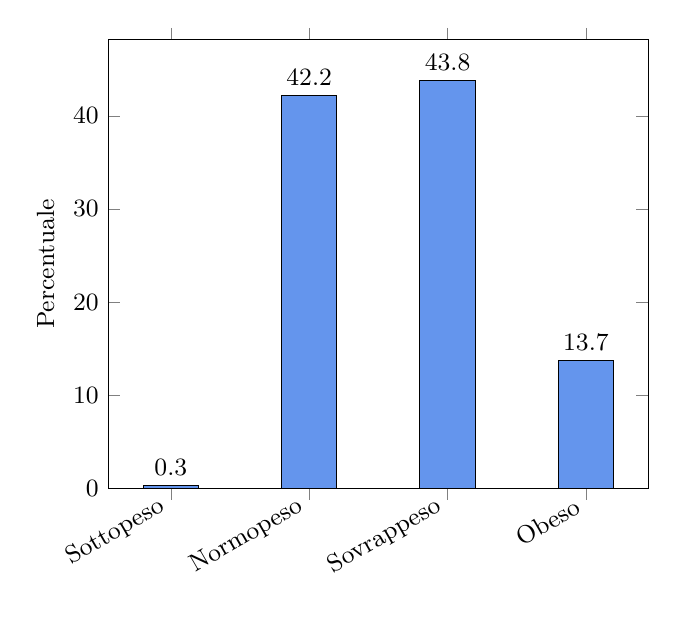
\begin{tikzpicture}[font=\small]
\begin{axis}[ymin=0,
ybar,
xtick=data,
ylabel=Percentuale,
x tick label style={rotate=30,anchor=east},
symbolic x coords={Sottopeso, Normopeso, Sovrappeso, Obeso},
bar width=20pt,enlarge x limits=0.15,nodes near coords,
nodes near coords align={vertical},
]
    \addplot[fill=CornflowerBlue,draw=black]
      coordinates{
	(Sottopeso, .3)
(Normopeso, 42.2)
(Sovrappeso, 43.8)
(Obeso,13.7)
      };
\end{axis}
\end{tikzpicture}

\end{esercizio}


\begin{esercizio}
\label{ese:4.23}
Eseguire le seguenti addizioni in base~3.

 % (c) 2012 Dimitrios Vrettos - d.vrettos@gmail.com
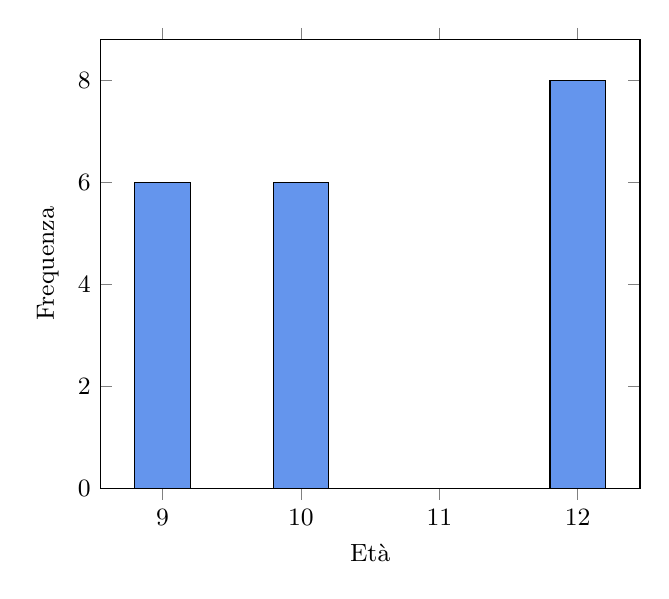
\begin{tikzpicture}[font=\small]

\begin{axis}[ymin=0,
ybar,
ylabel=Frequenza,
xlabel=Età,
bar width=20pt,
enlarge x limits=0.15,]

\addplot[fill=CornflowerBlue,draw=black]
      coordinates{
	(9, 6)
	(10,6)
	(12,8) };
\end{axis}
\end{tikzpicture}

\end{esercizio}

%%%%%%%%%%%%%%%%%%%%%%%%%%%%%%%%%%%%%%%%%%%%%
\begin{esercizio}
 \label{ese:4.24}
 Eseguire le seguenti sottrazioni in base~2.

 % (c) 2012 Dimitrios Vrettos - d.vrettos@gmail.com

\begin{tikzpicture}[x=10mm,y=10mm, font=\small,table nodes/.style={%
		rectangle,
		draw=black,
 		align=center,
   		minimum height=5mm,
     	text depth=0.5ex,
     	text height=1.5ex,
     	inner xsep=-1pt,
     	outer sep=0pt
	},
	table/.style={%
        matrix of nodes,
        row sep=-\pgflinewidth,
        column sep=-\pgflinewidth,
        nodes={%
            table nodes
        } }]

\matrix (first) [table,text width=7mm,name=table,row 2 column 2/.style=blue,row 5 column 4/.style=blue]
{
{}  & $-1$ & $+3$ & $-7$ & $+5$ & $-2$ & $+4$ & $+10$\\
$-1$ &[blue] 1 &{} &{} &{} &{} &{} &{} \\
$+3$ &{} &{} &{} &{} &{} &{} &{} \\
$-7$ &{} &{} &{} &{} &{} &{} &{} \\
$+5$ &{} &{} &{$0$} &{} &{} &{} &{} \\
$-2$ &{} &{} &{} &{} &{} &{} &{} \\
$+4$ &{} &{} &{} &{} &{} &{} &{} \\
$+10$ &{} &{} &{} &{} &{} &{} &{} \\
};

\end{tikzpicture}
\end{esercizio}

\begin{esercizio}
 \label{ese:4.25}
 Eseguire le seguenti sottrazioni in base~5.

 % (c) 2012 Dimitrios Vrettos - d.vrettos@gmail.com

\begin{tikzpicture}[x=10mm,y=10mm, font=\small, every state/.style={draw=CornflowerBlue}, every loop/.style={draw=Maroon}]
\draw (0,0) circle (2);
\node at (2,2) {$A$};
\node[state]  at (-1.5,0) {};
\node[state] (3) at (-.4,.8) {$+3$};
\node[state]  at (1.1,.5) {};
\node[state]  at (-.5,-.2) {};
\node[state] (10) at (1,-1) {$+10$};
\node[state] (7) at (-.5,-1.2) {$-7$};

\begin{scope}[->]
\path (3) edge[loop above] node{} ()
	(10) edge[loop above] node{} ()
   (7) edge[loop right] node {} ();

\end{scope}
\begin{scope}[-, Maroon]
\draw (10)--(3);
\end{scope}
\end{tikzpicture}
\end{esercizio}

\begin{esercizio}
 \label{ese:4.26}
 Eseguire le seguenti sottrazioni in base~3.

 % (c) 2012 Dimitrios Vrettos - d.vrettos@gmail.com
\begin{tikzpicture}[ anchor=north west]

\begin{scope}[nodes={ text centered },cells={anchor=south}]
\matrix(a) [matrix of nodes]
{
2&1&0&2&0&1&$-$ \\
{}&2&1&{2}&{1}&{2}\\
};
\draw(a-2-1.south west)--(a-2-6.south east);

\begin{scope}[xshift=31.3mm]
\matrix(b) [matrix of nodes]
{
2&0&2&1&0&1&$-$ \\
{}&{1}&{2}&{1}&{1}&{0}\\
};
\draw(b-2-1.south west)--(b-2-6.south east);
\end{scope}

\begin{scope}[xshift=62.6mm]
\matrix(c) [matrix of nodes]
{
2&2&1&1&$-$ \\
{}&2&0&2&\\
};
\draw(c-2-1.south west)--(c-2-4.south east);
\end{scope}

\begin{scope}[xshift=86mm]
\matrix(d) [matrix of nodes]
{
1&2&0&1&$-$ \\
{}&2&2&2&\\
};
\draw(d-2-1.south west)--(d-2-4.south east);
\end{scope}

\begin{scope}[xshift=109.3mm]
\matrix(e) [matrix of nodes]
{
2&1&0&0&1&$-$ \\
1&2&1&0&2&{}\\
};
\draw(e-2-1.south west)--(e-2-5.south east);
\end{scope}
\end{scope}

\end{tikzpicture}

\end{esercizio}

%%%%%%%%%%%%%%%%%%%%%%%%%%%%%%%%%%%%%%%%%%%%%%%

\begin{esercizio}
 \label{ese:4.27}
Moltiplicare in base~2:~\quad$111101_{2}\cdot~10110_{2}$;\quad
$101101_{2}\cdot~11111_{2}$;\quad~$1011_{2}\cdot~111_{2}$.
\end{esercizio}

\begin{esercizio}
 \label{ese:4.28}
Moltiplicare in base~5:~\quad$2401_{5}\cdot~42_{5}$;\quad
$431_{5}\cdot~34_{5}$;\quad~$214_{5}\cdot~41_{5}$.
\end{esercizio}

\begin{esercizio}
 \label{ese:4.29}
Moltiplicare in base~3:~\quad$10201_{3}\cdot~212_{3}$;\quad
$2101_{3}\cdot~212_{3}$;\quad~$1211_{3}\cdot~22_{3}$.
\end{esercizio}

\begin{esercizio}[\Ast]
\label{ese:4.30}
Eseguire le seguenti divisioni in base~2.
 \begin{multicols}{3}
 \begin{enumeratea}
  \item $11101_2:11_2$;
  \item $1011101_2:100_2$;
  \item $100011_2:10_2$.
 \end{enumeratea}
 \end{multicols}
\end{esercizio}

\begin{esercizio}[\Ast]
\label{ese:4.31}
Eseguire le seguenti divisioni in base~5.
 \begin{multicols}{3}
 \begin{enumeratea}
  \item $2304_5:43_5$;
  \item $3310_5:24_5$;
  \item $2012_5:31_5$.
 \end{enumeratea}
 \end{multicols}
\end{esercizio}

\subsection{Risposte}

\paragraph{\thechapter.3.} 29; 55; 203; 21; 653.

\paragraph{\thechapter.4.} 55; 9; 7; 63; 5.

\paragraph{\thechapter.5.} 527; 170; 25; 62.

\paragraph{\thechapter.20.} $667,57\unit{MiB}$.

\paragraph{\thechapter.30.}
a)~$\text{Q}=11_2$,~~$\text{R}=1_2$;\quad b)~$\text{Q}=1011_2$,~~$\text{R}=1_2$;\quad c)~$\text{Q}=10001_2$,~~$\text{R}=0_2$.

\paragraph{\thechapter.31.}
a)~$\text{Q}=24_5$,~~$\text{R}=12_5$;\quad b)~$\text{Q}=112_5$,~~$\text{R}=12_5$;\quad c)~$\text{Q}=31_5$,~~$\text{R}=1_5$.

\cleardoublepage
